
\section{Theorie}
\label{sec:Theorie}
In einem geschlossenen System mit zwei Wärmereservoiren unterschiedlicher Temperatur geht
  Wärmeenergie immer vom wärmeren zum kälteren Reservoir über, bis ein
  Temperaturausgleich zwischen beiden erfolgt ist. Um den Prozess
  umzukehren wird zusätzliche Energie benötigt. Ein Gerät, welches dies leistet,
  heißt Wärmepumpe.
 \subsection{Funktionsweise einer Wärmepumpe}
  \begin{figure}
  	\centering
  	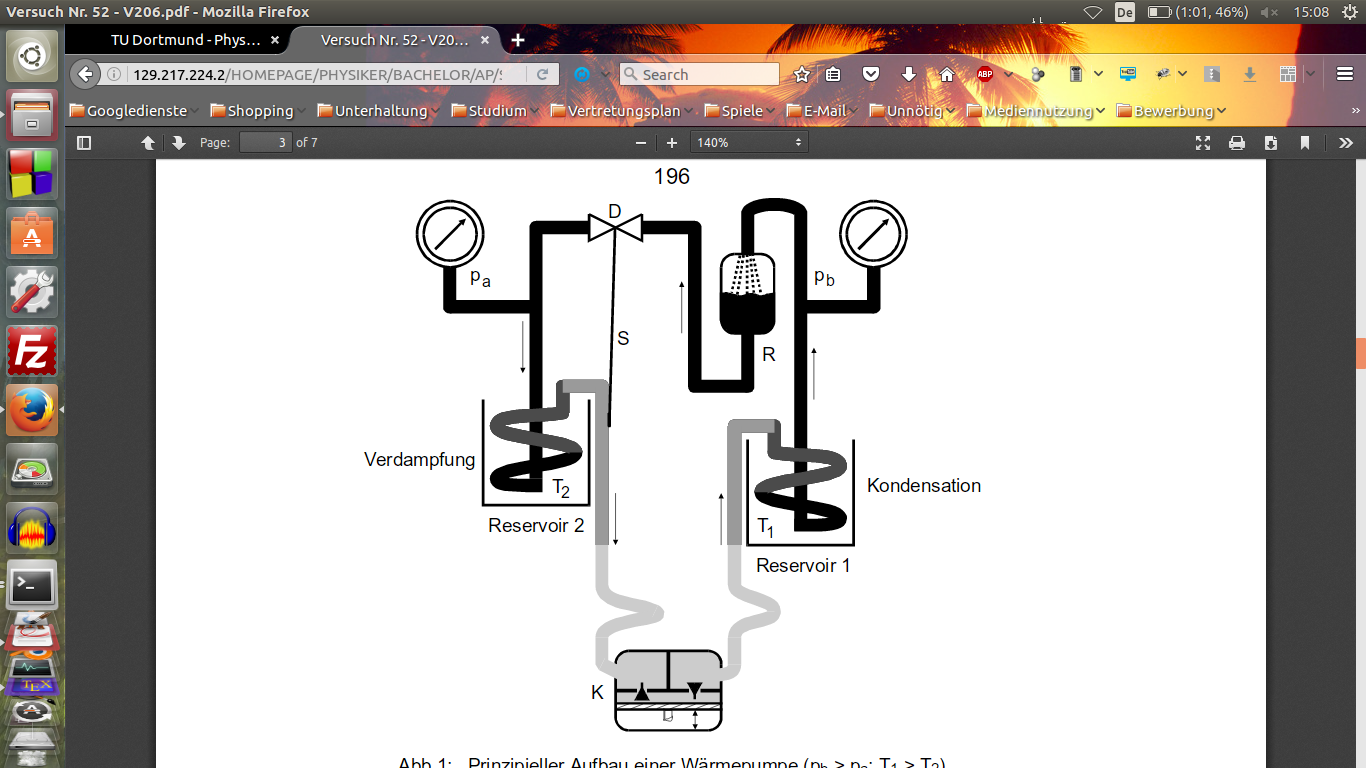
\includegraphics[width=\linewidth-100pt,height=\textheight-100pt,keepaspectratio]{content/Bilder/Aufbau.png}
  	\caption{Darstellung einer Wärmepumpe \cite{V206}.}
  	\label{fig:Aufbau1}
  \end{figure}
In Abbildung \ref{fig:Aufbau1} ist eine Wärmepumpe schematisch dargestellt.
Zum Wärmetransport wird ein reales Gas verwendet, welches verdampft,
wenn es die Verdampfungswärme $L$ pro Gramm im Reservoir 2 aufnimmt. Im Kompressor wird es dann nahezu adiabatisch komprimiert, sodass sich der Druck von $p_\text{a}$ auf $p_\text{b}$ erhöht und die Temperatur stark steigt. In Reservoir 1 verflüssigt sich das Gas aufgrund des größeren Druckes wieder, wobei es die Kondensationswärme $L$ pro Gramm wieder abgibt. Zuletzt durchströmt das flüssige Gas das Drosselventil $D$, wobei der Druck von $p_\text{b}$ wieder auf $p_\text{a}$ abfällt. Danach wiederholt sich der gesamte Prozess. Damit keine Gasblasen durch das Drosselventil $D$ gelangen, wird das flüssige Gas von den Gasbläschen in $R$ getrennt. Es muss zusätzlich noch der Massenstrom durch eine Steuervorrichtung $S$ am Drosselventil $D$ reguliert werden, damit keine Flüssigkeit in den Kompressor gelangt. 

\subsection{Die Güteziffer}
Für eine solche Wärmepumpe gilt nach dem 1. Hauptsatz der Wärmelehre die Bedingung
\begin{equation}
Q1 = Q2 + A\label{eq:Q1}\text{,}
\end{equation}
mit der an das wärmere Reservoir abgegeben Energie $Q1$, der dem kälteren
Reservoir entnommenen Energie $Q2$ und der zusätzlich benötigten Arbeit $A$.
Mithilfe dieses Zusammenhangs folgt die Güteziffer
\begin{equation}
v = \frac{Q1}{A}\label{eq:v1}\text{.}
\end{equation}
Da es sich im Idealfall um einen reversiblen Prozess handelt, folgt nach dem zweitem Hauptsatz für eine idealisierte Wärmepumpe
\begin{equation}
\frac{Q_1}{T_1}-\frac{Q_2}{T_2}=0\label{eq:redQ}\text{.}
\end{equation}
Damit folgt für die maximal erreichbare Güte
\begin{equation}
v = \frac{T1}{T1-T2}\label{eq:vid}\text{,}
\end{equation}
mit den Temperaturen $T1$ für das wärmere und $T2$ für das kältere Reservoir.
Da im realistischen Fall der Prozess nicht irreversibel ist, ist der Gütefaktor einer realen Wärmepumpe geringer.

Im folgendem wird die Güteziffer $v$, der in der späteren Messung verwendeten Wärmepumpe, die in Abbildung \ref{fig:Aufbau2} dargestellt ist, betrachtet. 

Für die durchschnittlich im Reservoir 1 pro Zeiteinheit zugeführte Wärmemenge gilt, mit der Wärmekapazität des Wassers $m_1c_\text{w}$ und des Kupferrohrs und Eimers $m_\text{k}c_\text{k}$
\begin{equation}
  \frac{\Delta Q1}{\Delta t} = \left( m_1c_\text{w} + m_\text{k}c_\text{k}\right) \frac{\Delta T_1}{\Delta t}\text{.}\label{eq:T1Q1}
\end{equation}
Mit $\Delta t= t_1 -t_0$ folgt die Beziehung
\begin{equation}
	v = \frac{\Delta Q_1}{\Delta A} =\frac{\Delta Q_1}{\int_{t_0}^{t_1} N_\text{mech} \diff t} = \frac{\Delta Q_1}{\Delta t \overline{N}}\text{,}
\end{equation}
wobei $N_\text{mech}$ die mechanische  Kompressorleistung und $\overline{N}=\frac{1}{\Delta t} \int_{t_0}^{t_1} N_\text{mech} \diff t$ die über den Zeitraum $\Delta t$ gemittelte Kompressorleistung ist.

\subsection{Der Massendurchsatz}
Es wird der Massendurchsatz der in der späteren Messung verwendeten Wärmepumpe, die in Abbildung \ref{fig:Aufbau2} dargestellt ist, betrachtet.

Analog zu Formel \eqref{eq:T1Q1} gilt für die durchschnittlich im Reservoir 2 pro Zeiteinheit entnommene Wärmemenge, mit der Wärmekapazität des Wassers $m_2c_\text{w}$ und des Kupferrohrs und Eimers $m_\text{k}c_\text{k}$
\begin{equation}
\frac{\Delta Q2}{\Delta t} = \left( m_2c_\text{w} + m_\text{k}c_\text{k}\right) \frac{\Delta T_2}{\Delta t}\text{.}\label{eq:T2Q2}\text{.}
\end{equation}
Es wird die Wärmemenge $\Delta Q_2$ durch verdampfen der Masse $\Delta m$ des Gases entnommen.
Es gilt mit der Verdampfungswärme $L$
\begin{equation}
\begin{aligned}
\Delta Q_2 = L \Delta m & \equiv & \frac{\Delta Q_2}{\Delta t} \cdot \frac{1}{L} = \frac{\Delta m}{\Delta t}\text{,}
\end{aligned}
\end{equation}
wobei $\frac{\Delta m}{\Delta t}$ der durchschnittliche Massendurchsatz in dem Zeitraum $\Delta t$ ist.

\subsection{Die mechanische Kompressorleistung}
Es wird die mechanische Kompressorleistung $N_\text{mech}$, des Kompressors aus der in der späteren Messung verwendeten Wärmepumpe, die in Abbildung \ref{fig:Aufbau2} dargestellt ist, betrachtet.

